\documentclass[class=minimal,border=1cm]{standalone}

\usepackage[svgnames]{xcolor}
\usepackage{tikz}
\usetikzlibrary{arrows,fit,positioning,shapes.arrows, shapes.geometric}
\usepackage{adjustbox}

\begin{document}

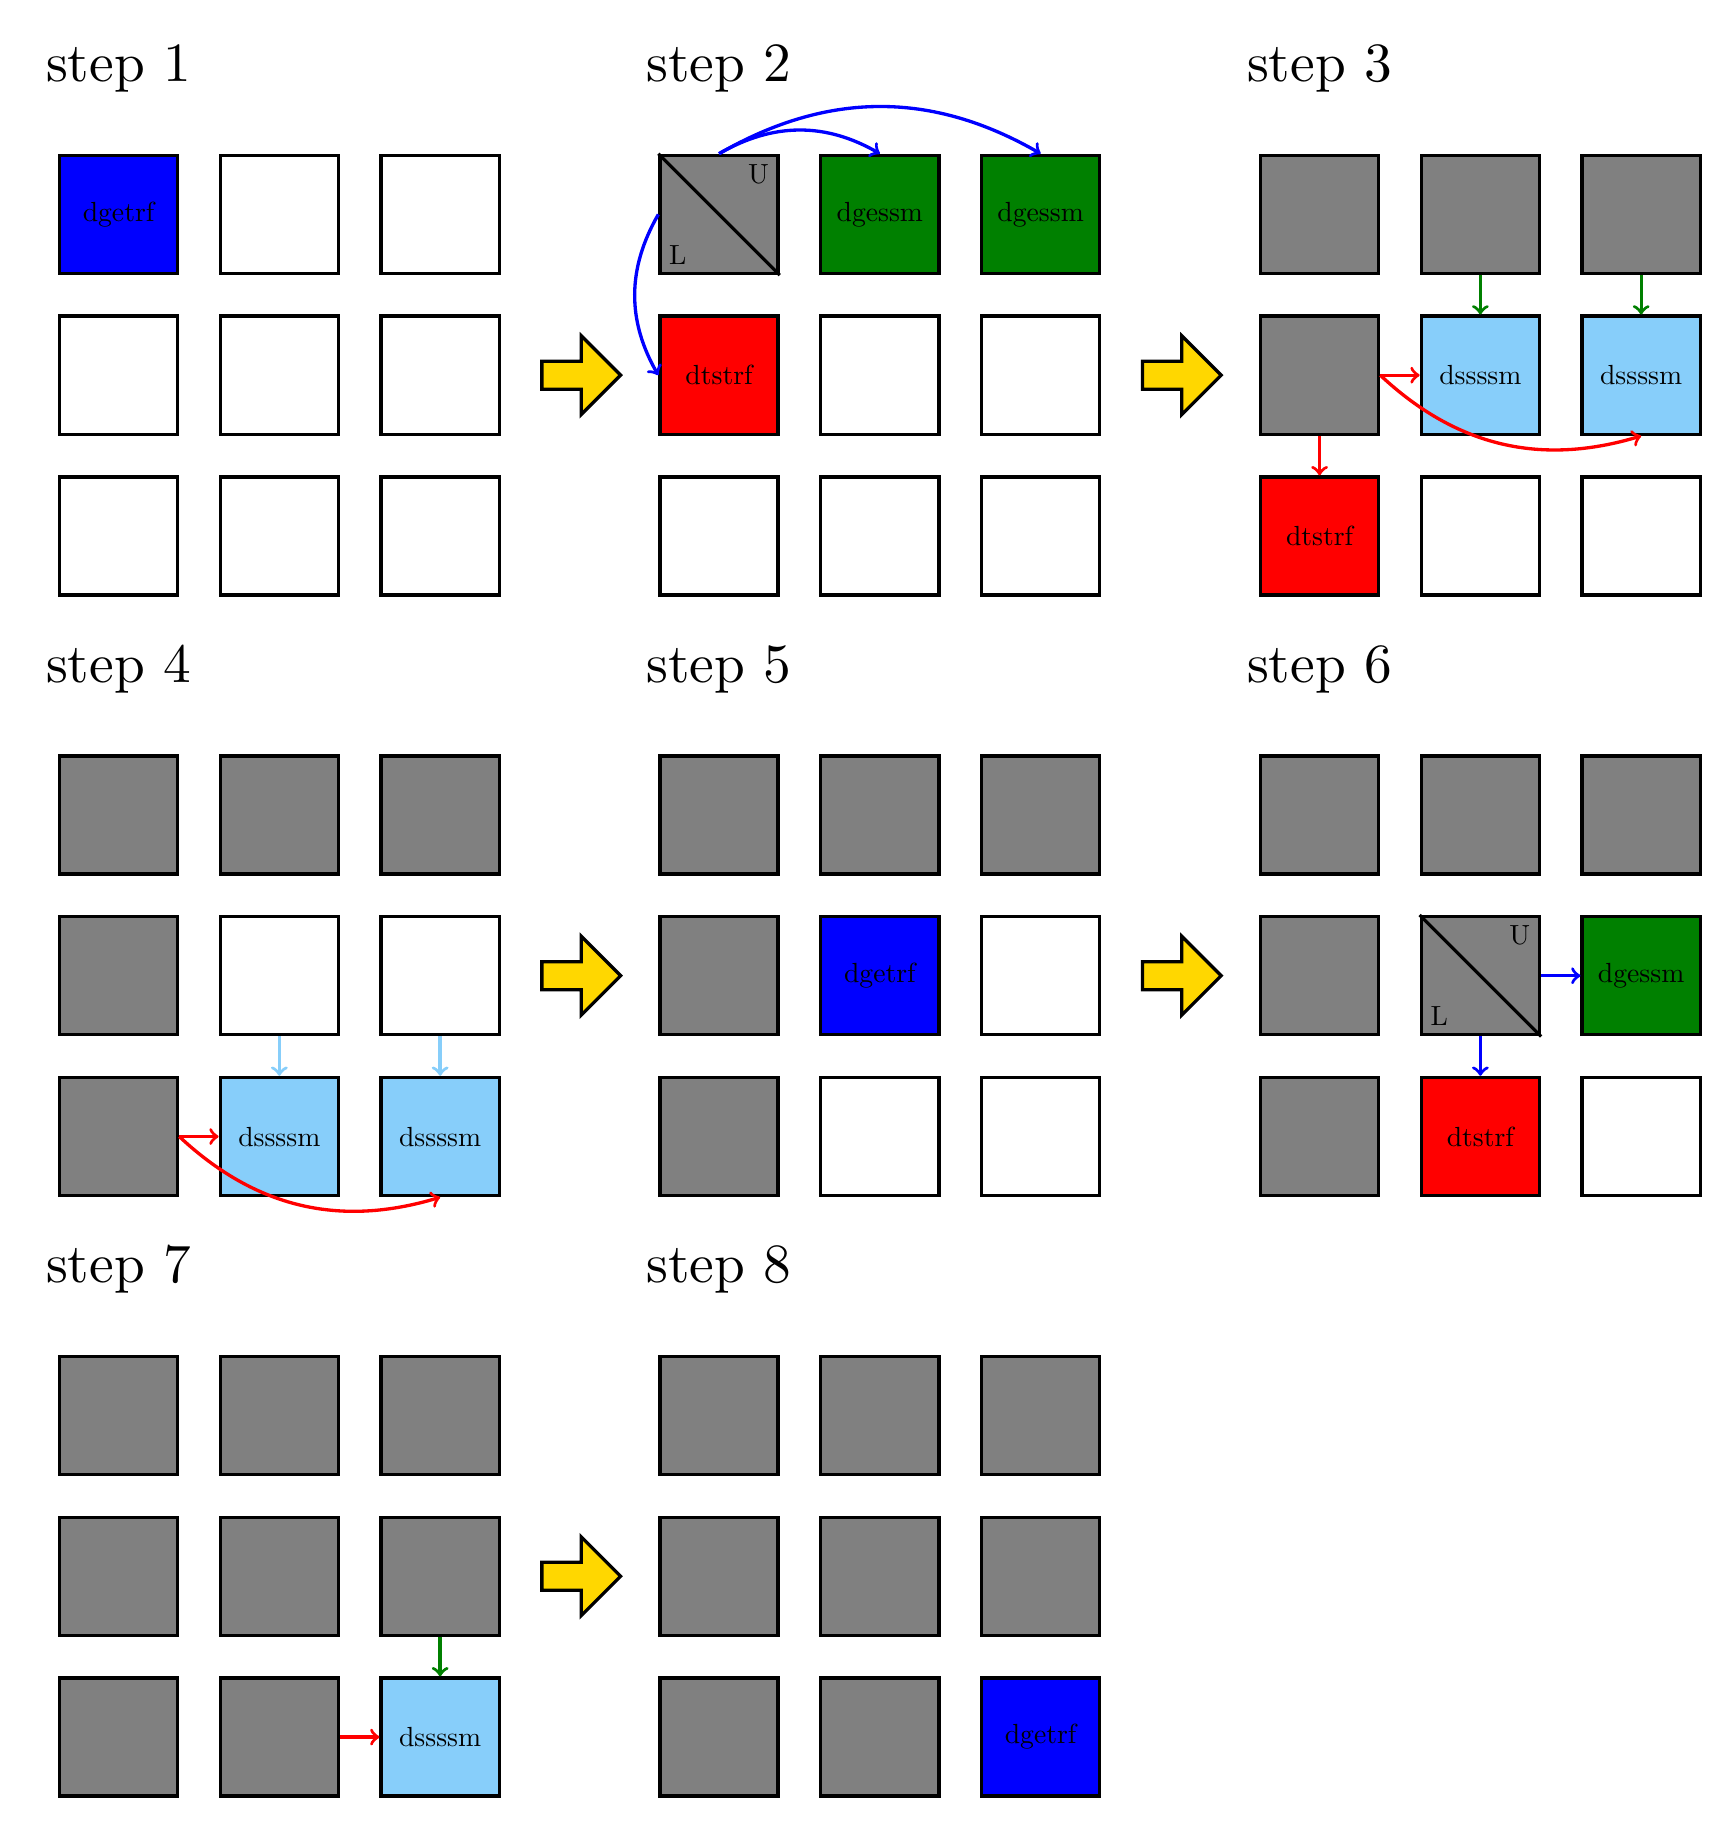
\begin{tikzpicture}[very thick,
block/.style={draw, minimum width=1.5cm, minimum height=1.5cm},
next_ar/.style={draw, single arrow, minimum width=1cm, minimum height=1cm, fill=Gold},
U_block/.style={draw, isosceles triangle, isosceles triangle apex angle=90, rotate=0, minimum width=2cm}]
	%k=1, step 1 
	\node[block, fill=Blue] (00_0) {dgetrf};
	\node[block, right=0.5cm of 00_0] (01_0) {};
	\node[block, right=0.5cm of 01_0] (02_0) {}; 

	\node[block, below=0.5cm of 00_0] (10_0) {};
	\node[block, below=0.5cm of 10_0] (20_0) {};  

	\node[block, right=0.5cm of 10_0] (11_0) {};
	\node[block, right=0.5cm of 11_0] (12_0) {};  
	\node[block, right=0.5cm of 20_0] (21_0) {};
	\node[block, right=0.5cm of 21_0] (22_0) {};

	\node[next_ar, right=0.5 of 12_0] {};

	%k=1, step 2
	\node[block, right=2cm of 02_0, fill=Gray] (00_1) {};
	\draw (00_1.north west) -- (00_1.south east);
  \node[anchor=north east] at (00_1.north east) (U_0) {U};
  \node[anchor=south west] at (00_1.south west) (L_0) {L};

	\node[block, right=0.5cm of 00_1, fill=Green] (01_1) {dgessm};
	\node[block, right=0.5cm of 01_1, fill=Green] (02_1) {dgessm}; 

	\node[block, below=0.5cm of 00_1, fill=Red] (10_1) {dtstrf};
	\node[block, below=0.5cm of 10_1] (20_1) {};  

	\node[block, right=0.5cm of 10_1] (11_1) {};
	\node[block, right=0.5cm of 11_1] (12_1) {};  
	\node[block, right=0.5cm of 20_1] (21_1) {};
	\node[block, right=0.5cm of 21_1] (22_1) {};

  \path[->, bend left, color=Blue] (00_1.north) edge (01_1.north);
	\path[->, bend left, color=Blue] (00_1.north) edge (02_1.north);
	\path[->, bend right, color=Blue] (00_1.west) edge (10_1.west);

	\node[next_ar, right=0.5 of 12_1] {};

	%k=1, step 3
	\node[block, right=2cm of 02_1, fill=Gray] (00_2) {};
	\node[block, right=0.5cm of 00_2, fill=Gray] (01_2) {};
	\node[block, right=0.5cm of 01_2, fill=Gray] (02_2) {}; 

	\node[block, below=0.5cm of 00_2, fill=Gray] (10_2) {};
	\node[block, below=0.5cm of 10_2, fill=Red] (20_2) {dtstrf};  

	\node[block, right=0.5cm of 10_2, fill=LightSkyBlue] (11_2) {dssssm};
	\node[block, right=0.5cm of 11_2, fill=LightSkyBlue] (12_2) {dssssm};  
	\node[block, right=0.5cm of 20_2] (21_2) {};
	\node[block, right=0.5cm of 21_2] (22_2) {};

	\path[->, color=Green] (01_2.south) edge (11_2.north);
	\path[->, color=Green] (02_2.south) edge (12_2.north);
	\path[->, color=Red] (10_2.east) edge (11_2.west);
	\path[->, bend right, color=Red] (10_2.east) edge (12_2.south);
	\path[->, color=Red] (10_2.south) edge (20_2.north);

	%k=1, step 4
	\node[block, below=2cm of 20_0, fill=Gray] (00_3) {};
	\node[block, right=0.5cm of 00_3, fill=Gray] (01_3) {};
	\node[block, right=0.5cm of 01_3, fill=Gray] (02_3) {}; 

	\node[block, below=0.5cm of 00_3, fill=Gray] (10_3) {};
	\node[block, below=0.5cm of 10_3, fill=Gray] (20_3) {};  

	\node[block, right=0.5cm of 10_3] (11_3) {};
	\node[block, right=0.5cm of 11_3] (12_3) {};  
	\node[block, right=0.5cm of 20_3, fill=LightSkyBlue] (21_3) {dssssm};
	\node[block, right=0.5cm of 21_3, fill=LightSkyBlue] (22_3) {dssssm};

	\path[->, color=LightSkyBlue] (11_3.south) edge (21_3.north);
	\path[->, color=LightSkyBlue] (12_3.south) edge (22_3.north);
	\path[->, color=Red] (20_3.east) edge (21_3.west);
	\path[->, bend right, color=Red] (20_3.east) edge (22_3.south);

	\node[next_ar, right=0.5 of 12_3] {};

	%k=2, step 1
	\node[block, right=2cm of 02_3, fill=Gray] (00_4) {};
	\node[block, right=0.5cm of 00_4, fill=Gray] (01_4) {};
	\node[block, right=0.5cm of 01_4, fill=Gray] (02_4) {}; 

	\node[block, below=0.5cm of 00_4, fill=Gray] (10_4) {};
	\node[block, below=0.5cm of 10_4, fill=Gray] (20_4) {};  

	\node[block, right=0.5cm of 10_4, fill=Blue] (11_4) {dgetrf};
	\node[block, right=0.5cm of 11_4] (12_4) {};  
	\node[block, right=0.5cm of 20_4] (21_4) {};
	\node[block, right=0.5cm of 21_4] (22_4) {};

	\node[next_ar, right=0.5 of 12_4] {};

	%k=2, step 2
	\node[block, right=2cm of 02_4, fill=Gray] (00_5) {};
	\node[block, right=0.5cm of 00_5, fill=Gray] (01_5) {};
	\node[block, right=0.5cm of 01_5, fill=Gray] (02_5) {}; 

	\node[block, below=0.5cm of 00_5, fill=Gray] (10_5) {};
	\node[block, below=0.5cm of 10_5, fill=Gray] (20_5) {};  

	\node[block, right=0.5cm of 10_5, fill=Gray] (11_5) {};
	\draw (11_5.north west) -- (11_5.south east);
  \node[anchor=north east] at (11_5.north east) (U_1) {U};
  \node[anchor=south west] at (11_5.south west) (L_1) {L};

	\node[block, right=0.5cm of 11_5, fill=Green] (12_5) {dgessm};  
	\node[block, right=0.5cm of 20_5, fill=Red] (21_5) {dtstrf};
	\node[block, right=0.5cm of 21_5] (22_5) {};

	\path[->, color=Blue] (11_5.east) edge (12_5.west);
	\path[->, color=Blue] (11_5.south) edge (21_5.north);

	%k=2, step 3
	\node[block, below=2cm of 20_3, fill=Gray] (00_6) {};
	\node[block, right=0.5cm of 00_6, fill=Gray] (01_6) {};
	\node[block, right=0.5cm of 01_6, fill=Gray] (02_6) {}; 

	\node[block, below=0.5cm of 00_6, fill=Gray] (10_6) {};
	\node[block, below=0.5cm of 10_6, fill=Gray] (20_6) {};  

	\node[block, right=0.5cm of 10_6, fill=Gray] (11_6) {};

	\node[block, right=0.5cm of 11_6, fill=Gray] (12_6) {};  
	\node[block, right=0.5cm of 20_6, fill=Gray] (21_6) {};
	\node[block, right=0.5cm of 21_6, fill=LightSkyBlue] (22_6) {dssssm};

	\path[->, color=Green] (12_6.south) edge (22_6.north);
	\path[->, color=Red] (21_6.east) edge (22_6.west);

	\node[next_ar, right=0.5 of 12_6] {};

	%k=2, step 4
	\node[block, right=2cm of 02_6, fill=Gray] (00_7) {};
	\node[block, right=0.5cm of 00_7, fill=Gray] (01_7) {};
	\node[block, right=0.5cm of 01_7, fill=Gray] (02_7) {}; 

	\node[block, below=0.5cm of 00_7, fill=Gray] (10_7) {};
	\node[block, below=0.5cm of 10_7, fill=Gray] (20_7) {};  

	\node[block, right=0.5cm of 10_7, fill=Gray] (11_7) {};

	\node[block, right=0.5cm of 11_7, fill=Gray] (12_7) {};  
	\node[block, right=0.5cm of 20_7, fill=Gray] (21_7) {};
	\node[block, right=0.5cm of 21_7, fill=Blue] (22_7) {dgetrf};

	%extra
	\node[above=0.5cm of 00_0, scale=2] {step 1};
	\node[above=0.5cm of 00_1, scale=2] {step 2};
	\node[above=0.5cm of 00_2, scale=2] {step 3};
	\node[above=0.5cm of 00_3, scale=2] {step 4};
	\node[above=0.5cm of 00_4, scale=2] {step 5};
	\node[above=0.5cm of 00_5, scale=2] {step 6};
	\node[above=0.5cm of 00_6, scale=2] {step 7};
	\node[above=0.5cm of 00_7, scale=2] {step 8};

\end{tikzpicture}

\end{document}
